\documentclass{scrartcl}

% packages
\usepackage{amsmath}
\usepackage{amssymb}
\usepackage[ngerman]{babel}
\usepackage{booktabs}
\usepackage[font=small,labelfont=bf]{caption}
\usepackage{csquotes}
\usepackage{float}
\usepackage{fontspec}
  \setmainfont[Ligatures=TeX]{Tex Gyre Pagella}
\usepackage{graphicx}
 \usepackage[pdfusetitle,unicode]{hyperref}
\usepackage{mathtools}
\usepackage{microtype}
\usepackage{siunitx}
  \sisetup{separate-uncertainty=true}
\usepackage{subcaption}
\usepackage[math-style=ISO,bold-style=ISO]{unicode-math}
  %\setmathfont{"[Tex Gyre Pagella Math.ttf]"}
\usepackage{xfrac}

% options
\setlength{\parindent}{0pt}  % no stupid indentation

% commands
\DeclarePairedDelimiter{\abs}{\lvert}{\rvert}
\DeclarePairedDelimiter{\mean}{\langle}{\rangle}
\renewcommand{\vec}[1]{\mathbf{#1}}
\renewcommand{\i}{\mathrm{i}}
\DeclareRobustCommand{\e}{\ensuremath{\mathrm{e}}}

% meta
\author{Kevin Dungs \and Kevin Heinicke}
\title{Computational Physics}
\subtitle{Übungsblatt 2}

% document
\begin{document}
\maketitle

\section*{Hausaufgabe 6: Site-Perkolation auf dem Quadratgitter}

Für diese Aufgabe haben wir zwei verschiedene Implementierungen gewählt. Die folgenden Ergebnisse sind mittels
\texttt{Forest.h} erstellt worden. Einen weiteren Ansatz liefert \texttt{union\_find.h}.

\subsection*{Visualisierung der Cluster}

Plots verschieden großer Cluster bei verschiedenen $p$ können durch \texttt{make plots} erstellt werden. 

\begin{figure}[H]
    \centering
    \begin{subfigure}{.31\textwidth}
        \centering
        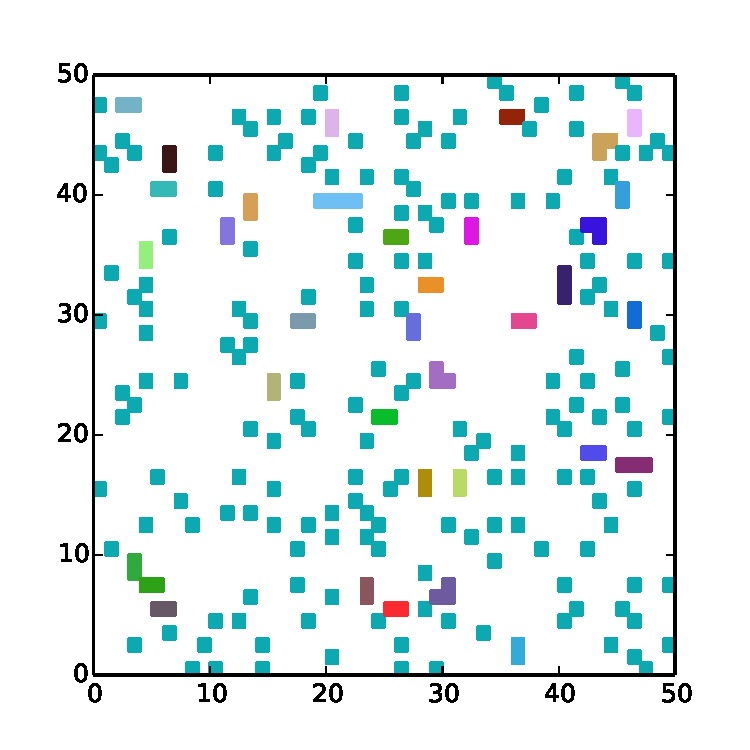
\includegraphics[width=\textwidth]{plots/50-01.pdf}
    \end{subfigure}
    \begin{subfigure}{.31\textwidth}
        \centering
        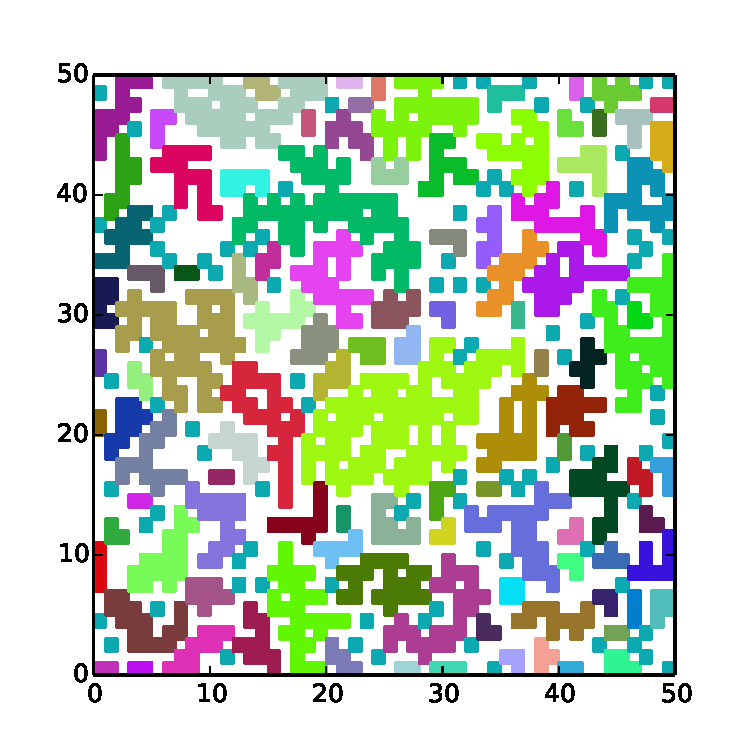
\includegraphics[width=\textwidth]{plots/50-05.pdf}
    \end{subfigure}
    \begin{subfigure}{.31\textwidth}
        \centering
        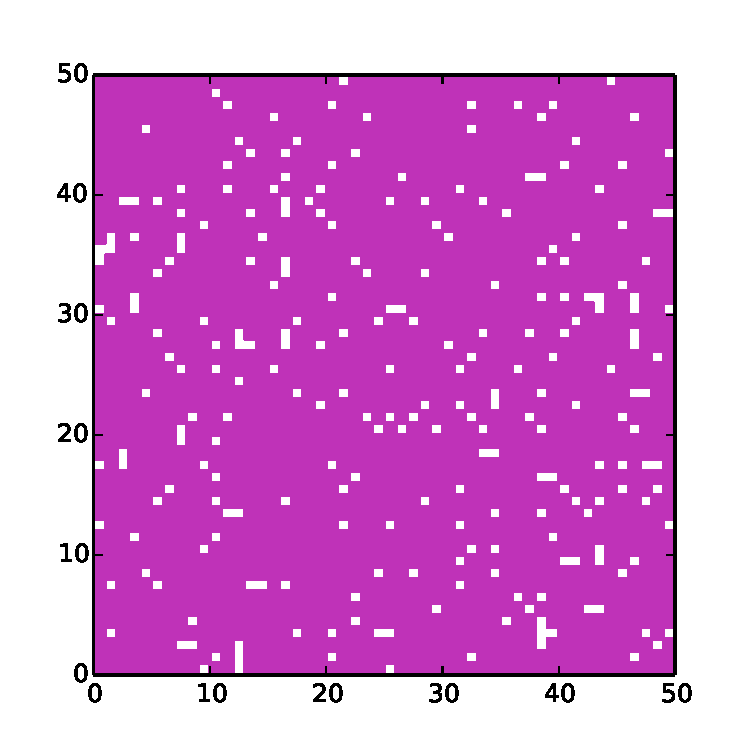
\includegraphics[width=\textwidth]{plots/50-09.pdf}
    \end{subfigure}
\end{figure}

\newpage

\subsection*{Bestimmung von $p_c$ und $b$}

Mittels \texttt{make fit} werden $p_c$ und $\beta$ bestimmt.

\begin{figure}[H]
    \centering
    \begin{subfigure}{.48\textwidth}
        \centering
        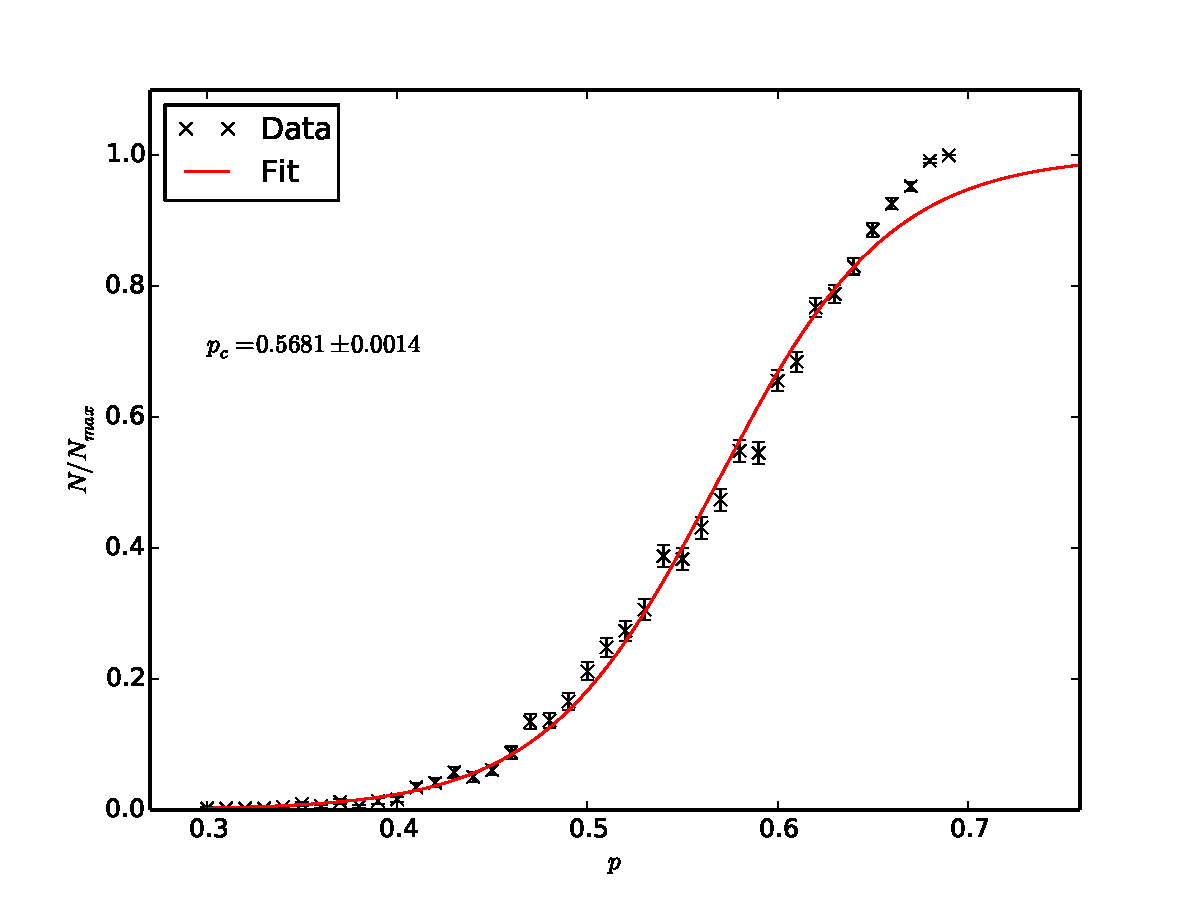
\includegraphics[width=\textwidth]{plots/p10.pdf}
    \end{subfigure}
    \begin{subfigure}{.48\textwidth}
        \centering
        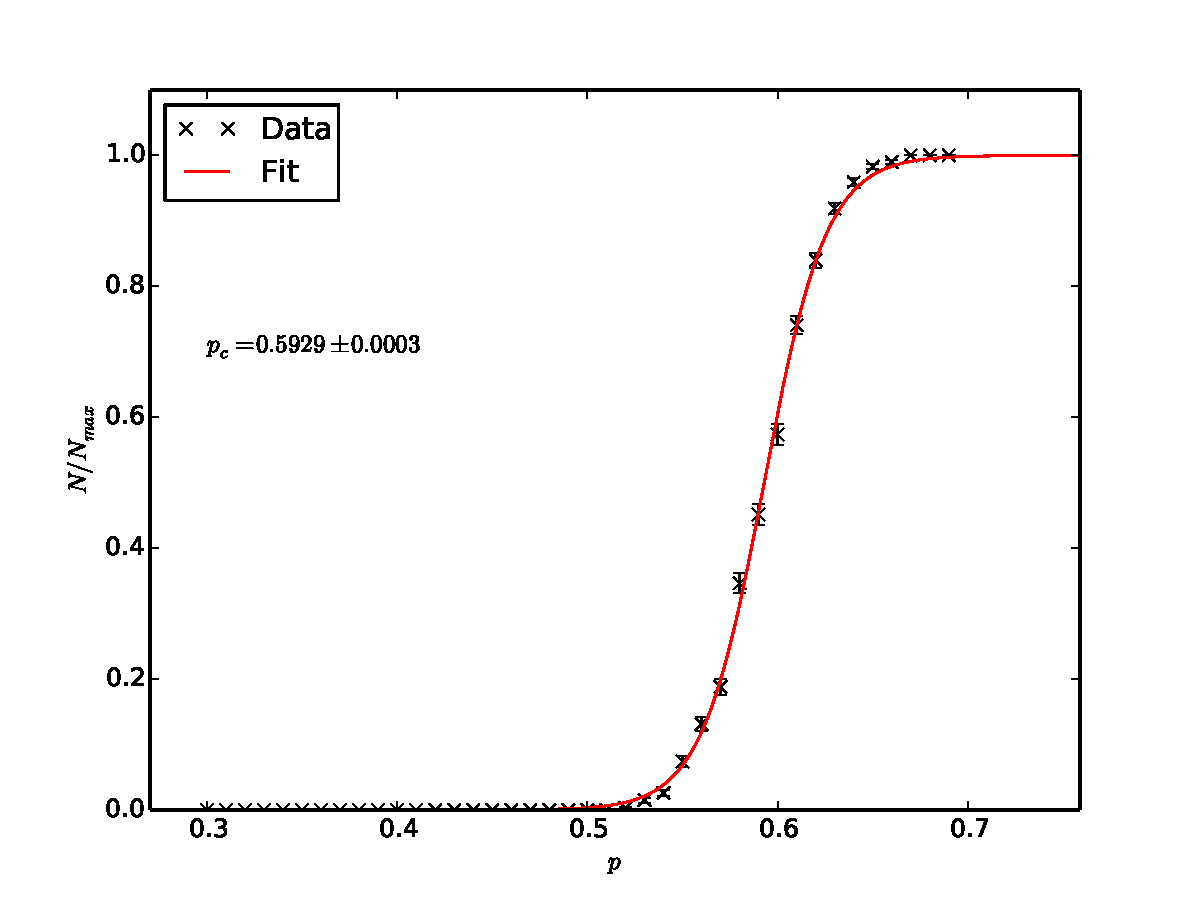
\includegraphics[width=\textwidth]{plots/p50.pdf}
    \end{subfigure}
    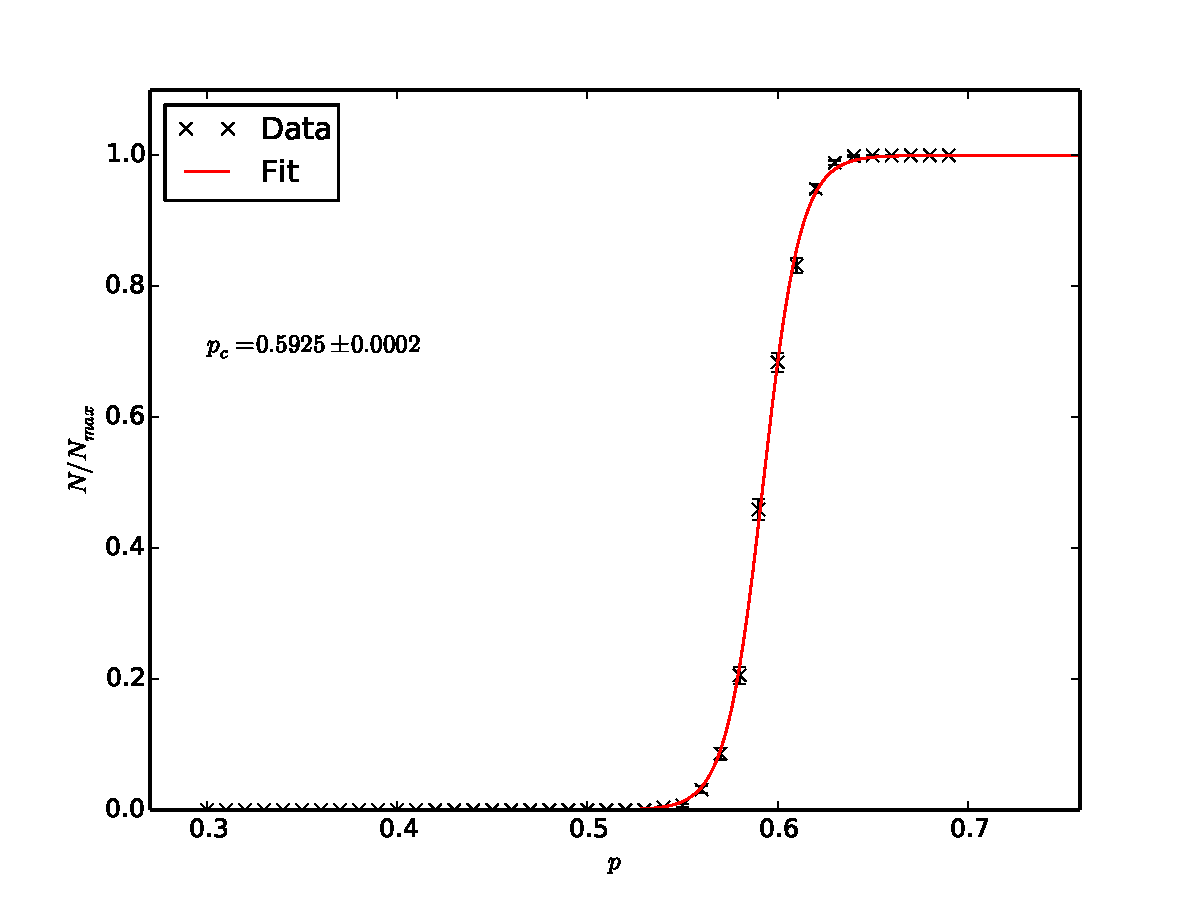
\includegraphics[width=10cm]{plots/p100.pdf}
\end{figure}

Die Werte schwanken dabei um

\begin{eqnarray*}
    p_c & = & \SI{0.597(2)}{} \\
    \beta & = & \SI{1.0}{}
\end{eqnarray*}

Bei der Bestimmung von $\beta$ wurden alle Werte $p > p_c$ ignoriert,
da die Größe des Gitter ab hier offensichtlich beschränkt. 

\end{document}
